\documentclass[10pt,a4paper]{article}
\renewcommand{\baselinestretch}{1}
\usepackage{amssymb,amsmath}            
\usepackage{graphicx}                   
\usepackage{indentfirst}
\usepackage{microtype}
\usepackage{moreverb}
\usepackage{multicol}
\usepackage{hyperref}
\usepackage[margin=1.2in]{geometry}

\title{Introduction to Vision and Robotics - Coursework 1 Report}           
\author{Milan Pavlik, Victor Dumitrescu}                      
\date{7th March 2014}                 

\begin{document}
\maketitle  % this inserts title, author info
%

\begin{multicols}{2}

\section{Introduction}

The purpose of this report is to outline the task at hand, the techniques and approaches used to produce a solution and a discussion of the results obtained on various datasets.

\subsection{The task}

The main idea of the task is to detect moving objects in a video sequence. Objects are thrown into the air and the goal is to distinguish between objects that are balls and the rest. This is similar to the famous mobile application Fruit Ninja where the user is required to slice all fruits but avoid touching anything else.



\subsection{Main ideas}

\paragraph{Background Model}
In order to create a background model for the video sequence, a Gaussian Mixture based Foreground Detector (FD) is used. It creates a background model of the image sequence by considering two Gaussian models where one models the moving objects that later appear in the sequence. The other one is used to model the background \cite{ES1}.
The technique considers each pixel separately and calculates the probability it belongs into one of the three Gaussians. The highest probability Gaussian is then assigned to that that pixel. The overall result obtained is assignment to three different classes where the object class represents the object in the video. 

\paragraph{Blob Analysis}
The \texttt{BlobAnalysis} object in Matlab works on the basis of forming a boundary around the object in question based on local continuity. It encapsulates the method for easier use and allows us to extract information from the mask produced by the Foreground Detector. It provides information such as area, centroid, bounding box, major and minor axis, eccentricity and perimeter to be used for object classification.

\paragraph{Kalman Filter}
Kalman filter is a model used to predict the positions of object that are inherently subject to noise. It is a recursive algorithm which works in two phases:

\begin{enumerate}
\item Predict - the expected location at time \textit{t+1} is returned based on physics models of constant velocity and constant acceleration.
\item Correct - the actual value observed is supplied. The algorithm adjusts its prediction based on the actual value and attempts to improve accuracy of the next prediction.
\end{enumerate}

Despite the balls being thrown into the air do not have constant velocity and constant acceleration it allows us to make a reasonable prediction of the next location.

\subsection{Research}

\paragraph{} The final version submitted for this assignment is based on Mathworks' tutorial on {\itshape Motion-Based Multiple Object Tracking \cite{ES2}}. We have researched the methods described and we used the provided code as the starting point for our object detection and tracking algorithms. We have optimized our solution for this particular task and added the functionality required for correct object classification and determining the highest point.
\paragraph{}	The main reason for using the techniques described in the tutorial was recognition speed. Our first attempts, involving background subtraction and normalisation, were performing considerably slower than the implementation based on Matlab's Vision toolkit.

\end{multicols}

\section{Methods}

\subsection{Object detection}
	
Object detection is done in stages. Firstly, all blobs in an image are analyzed using Blob Analysis and returned for further analysis. The code handling the blob analysis appears below inside the function \texttt{detectObjects()}:

\begin{verbatimtab}
function [areas, centroids, bboxes, mask, majora, ...
          minora, eccentricities, perimeters] = detectObjects(frame)
        % Detect foreground.
        mask = obj.detector.step(frame);

        % Perform blob analysis to find connected components.
        [areas, centroids, bboxes, majora, minora, ...
        eccentricities, perimeters] = obj.blobAnalyser.step(mask);
    end
\end{verbatimtab}

We step through the frame and create a mask for the current frame. This frame is then passed into the Blob Analysis object inside Matlab's vision toolkit. We obtain a list of object properties which is passed back to the main program loop. 

\subsection{Object tracking and representation}

In order to link objects in consecutive frames we use Kalman Filter to obtain the expected location of a frame. This allows us to distinguish two objects moving from each side of the frame upwards and towards each other. The Kalman filter gives us the predicted position of the objects in the current frame based on the previous frame. This approach is less expensive than comparing the shape properties and the average color of each blob between frames to link the detections together. We achieve the prediction in the following bit of code:

\begin{samepage}
\begin{verbatimtab}
function predictNewLocationsOfTracks()
	for i = 1:length(tracks)
		bbox = tracks(i).bbox;

		% Predict the current location of the track.
		predictedCentroid = predict(tracks(i).kalmanFilter);

		% Shift the bounding box so that its center is at
		% the predicted location.
		predictedCentroid = int32(predictedCentroid) - bbox(3:4) / 2;
		tracks(i).bbox = [predictedCentroid, bbox(3:4)];
	end
end
\end{verbatimtab}
\end{samepage}

The secondary benefit of using a Kalman filter is that lost objects can still be tracked for a reasonable amount of time and masking problems between consecutive frames are minimized.
	We then proceed to assign our detections to tracks. This is done using the Hungarian assignment algorithm, respectively a modified version of it. In order to compute this function, we first need to determine the cost of assignment and the cost of non-assignment to the current tracks.
	
\begin{enumerate}
\item Cost of assignment - the most straight forwards approach is used where the Cartesian distance between two points is taken. That is, the distance between the prediction and the actual centroid of a point. This is done in the following bit of code:
	\begin{samepage}
	\begin{verbatimtab}
% Compute the cost of assigning each detection to each track.
cost = zeros(nTracks, nDetections);
for i = 1:nTracks
	cost(i, :) = distance(tracks(i).kalmanFilter, centroids);
end
	\end{verbatimtab}
	\end{samepage}
\item Cost of non-assignment - this is the cost the Hungarian algorithm will use for its heuristics to estimate our assignment. We have determined the value of 20 to work the best based on observation.
\end{enumerate}

In the next step we compute the assignment and obtain an assignment to tracks, new tracks and tracks that are no longer visible in the frame.

\begin{samepage}
\begin{verbatimtab}
[assignments, unassignedTracks, unassignedDetections] = ...
	assignDetectionsToTracks(cost, costOfNonAssignment);
\end{verbatimtab}
\end{samepage}

The next step is to update information about the tracks that have indeed been assigned. We consider this in the \texttt{updateAssignedTracks()} function. First we loop over all the assignments and update its information stored in a struct. This information involves the bounding box, the age of the track, it's highest point so far and information about whether we have reached the highest point and should stop (described below).
	In the remain steps of tracking we generally concern ourselves with housekeeping. This involves incrementing the age of all unassigned tracks to be potentially deleted from the list of tracks in the next step. This happens inside the \texttt{updateUnassignedTracks()} function shown below:

\begin{samepage}
\begin{verbatimtab}
function updateUnassignedTracks()
	for i = 1:length(unassignedTracks)
		ind = unassignedTracks(i);
		tracks(ind).age = tracks(ind).age + 1;
		tracks(ind).consecutiveInvisibleCount = ...
			tracks(ind).consecutiveInvisibleCount + 1;
	end
end
\end{verbatimtab}
\end{samepage}

Next, we delete all unassigned tracks that are too old. This improves the space complexity and cleans up the tracks. We delete all tracks that have a visibility ratio of less than 0.6, or have been seen less than 0.6 of the time they are present in the tracks. The value of 0.6 works well by observation.

%\begin{samepage}
\begin{verbatimtab}
function deleteLostTracks()
	if isempty(tracks)
		return;
	end

	invisibleForTooLong = 4;
	ageThreshold = 8;

	% Compute the fraction of the track's age for which it was visible.
	ages = [tracks(:).age];
	totalVisibleCounts = [tracks(:).totalVisibleCount];
	visibility = totalVisibleCounts ./ ages;

	% Find the indices of 'lost' tracks.
	lostInds = (ages < ageThreshold & visibility < 0.6) | ...
		[tracks(:).consecutiveInvisibleCount] >= invisibleForTooLong;

	% Delete lost tracks.
	tracks = tracks(~lostInds);
end
\end{verbatimtab}
%\end{samepage}

Finally,  we create new tracks from the tracks that remain, that is tracks that are not too old to be deleted and have not been assigned to previous tracks. This is done inside the \texttt{createNewTracks()} function shown below:

%\begin{samepage}
\begin{verbatimtab}
function createNewTracks()
	centroids = centroids(unassignedDetections, :);
	bboxes = bboxes(unassignedDetections, :);

	for i = 1:size(centroids, 1)

		centroid = centroids(i,:);
		bbox = bboxes(i, :);

		% Create a Kalman filter object.
		kalmanFilter = configureKalmanFilter('ConstantVelocity', ...
			centroid, [200, 50], [100, 25], 100);

		% Create a new track.
		newTrack = struct(...
			'id', nextId, ...
			'bbox', bbox, ...
			'kalmanFilter', kalmanFilter, ...
			'age', 1, ...
			'totalVisibleCount', 1, ...
			'consecutiveInvisibleCount', 0, ...
			'stack', java.util.ArrayList(), ...
			'max_x', -1, ...
			'max_y', Inf, ...
			'last_x', -1, ...
			'last_y', Inf, ...
			'should_pause', false, ...
			'stop_pausing', false, ...
			'track_xs', java.util.ArrayList(), ...
			'track_ys', java.util.ArrayList());

		% Add it to the array of tracks.
		tracks(end + 1) = newTrack;

		% Increment the next id.
		nextId = nextId + 1;
	end
\end{verbatimtab}
%\end{samepage}

The benefit of creating tracks this way means that we have eliminated all other possibilities before make the decision to create a new object to track.

\subsection{Determining highest point}

\paragraph{} The highest point detection of an object thrown in the air is based on the gradient change in each frame relative to the previous frame. The idea is taken from calculus where the highest point of a downwards shaped parabola is when the gradient is zero. 
\paragraph{} In practice, to find the highest point a ball reaches, we look at the y coordinate of the point top middle point of the bounding box for a track. We made the assumption that the highest point is not the centroid but the middle point. In Matlab, pixels of an image are indexed from the top left corner which means we are actually searching for the smallest y coordinate of an object.
\paragraph{} We take the approach of keeping track of the lowest y coordinate so far and update this value whenever we visit the next frame. In code it translates to the following:

\begin{samepage}
\begin{verbatimtab}
	% Re-assign values if current max
	if y < tracks(idx).max_y
		tracks(idx).max_x = x;
		tracks(idx).max_y = y;
	end
\end{verbatimtab}
\end{samepage}

\paragraph{} Tracks is a matrix of structs containing information about each track and idx is just a looping index. The snippet causes our maximum value to update to the current value of x and y - the centroid. This way, the value is incrementally updated up until the point we reach the maximum.
\paragraph{} We also calculate the difference between the y coordinates in the last two frames. This gives us the change in coordinates and allows us to determine whether a ball is moving up or down. The following code performs the task:

\begin{samepage}
\begin{verbatimtab}
	% Calculate delta - the change in y coordinates
	% If checks are to exclude newly initialized objects.
	if tracks(idx).last_y ~= Inf && tracks(idx).last_y ~= -1
		deltaY = tracks(idx).last_y - y;
	else
		deltaY = 1;
	end
\end{verbatimtab}
\end{samepage}

\paragraph{} We set \texttt{deltaY} to 1 if we are currently looking at a newly initialized object that has just entered the frame. The following step is to either mark the object to be paused after the highest point marker has been drawn in the GUI or not. This is done in the following snippet:

\begin{samepage}
\begin{verbatimtab}
if deltaY < 0 && ~reached_highest.contains(idx)
	% Only pause if the probabilty of being a ball given the past 
	% is past the threshold
	if getBallProbability(tracks(idx).stack) > ball_probability_threshold
		tracks(idx).should_pause = true;
	else
		if ~reached_highest.contains(tracks(idx).id)
			reached_highest.add(tracks(idx).id);
		end
	end
end
\end{verbatimtab}
\end{samepage}

\paragraph{} First we check that the object has started falling down and that we have not yet paused for this object, this is done on the first line with \texttt{reached\_highest} and uses a \texttt{java.util.ArrayList()} to keep track of the objects we have stopped for. Checking that the object has started falling down gives us the advantage of robustness against sudden change in the size of the track to a smaller. We then proceed to calculate the probability that an object is a ball (explained later) and only pause if an object is categorized as a ball. Finally, we do a bit of housekeeping and add the object to the list of points that have reached its highest point and should not be paused for again.

\paragraph{} The method presented for finding the highest point only considers the current frame compared to the last frame and does not require any look ahead or extensive history of the points location.

\subsection{Ball recognition}

\paragraph{} Before discussing the actual algorithm used for classification, we will outline the general method. Once an object is detected and tracked, it is represented using a \texttt{struct} which contains its properties. In each frame, the \texttt{isBall()} method is applied on each object, returning a boolean. 
\paragraph{} These decisions are all stored in the object \texttt{struct}. Once enough frames have been analysed, we compute the ratio of frames where the object was classified as a ball compared to the total number of frames. This ratio is displayed next to each object. When it reaches the highest point, we compare this ratio to out ball recognition probability threshold (determined experimentally) in order to decide whether to pause or not.
\paragraph{} Before attempting to manually implement any complex methods, we thought that we might be able to exploit some of the properties that are computed by Matlab's \texttt{BlobAnalysis} module, applied to our binary mask. Provided that our masking is done correctly, this should offer accurate information about a blob. Among other computations, it calculates the normalized second central moment of each blob and returns the major and minor axis lengths of the ellipses that would fit them. It also provides the eccentricity of each of these ellipses.
\paragraph{} Our method consists of a series of nested if statements. At each step, the blob can either be declared as not a ball, or go forward with the next check. These are, in order, the checks that we apply:

\begin{enumerate}
\item The eccentricity of the ellipse (described above) has to be below 0.8 in order to indicate a roughly circular shape. If the blob is too elongated, we assume it cannot be a ball.
\item An estimated radius of the blob is computed, by averaging the lengths of the ellipse's axes. This is used to calculate the estimated perimeter and compare it to the actual perimeter of the blob, as returned by the \texttt{BlobAnalysis}. We have determined that if their ratio is greater than 1.2 then the object can no longer be considered to be a ball.
\item Compactness, the last check, has a threshold of 1.8 (again, determined by observation). It is also computed from the properties output by \texttt{BlobAnalysis}, namely perimeter and area.
\end{enumerate}
\paragraph{} Before deciding to use compactness, we have also experimented with not actually having a third check. This worked fairly well, but it resulted in quite a high number of cubes being classified as balls. We then tried corner detection. Although this solved the cube misclassifications, it also increased the number of (mostly large) balls that were misclassified. In the end, we settled for compactness, which results in a better compromise between the two extremes described above.

\paragraph{Ball probability} In order to increase robustness, we have added a list to each object we track keeping track of the whether the current object (described above) is likely to be a ball or not (as mentioned above). The values are then revisited in each frame and total count of true values is made. The probability that the object we are tracking is a ball is then the ratio of true to false or \texttt{true\_count / total\_size}. The function \texttt{getBallProbability(stack)} handles this approach. Additionally, for increased robustness we only consider lists of minimum length eight. The assumption is throwing a ball in the air will take at least a few frames to reach its highest point. By observation, we determined the value of eight to be suitable for this task.


\section{Results}

\subsection{Object detection}
The binary masking that we use to isolate the blobs does a very good job. It almost always discriminates correctly between background and objects. The blob generally correspond perfectly with the shape of the object. There are a few, rarely occurring exceptions:

\begin{center}
  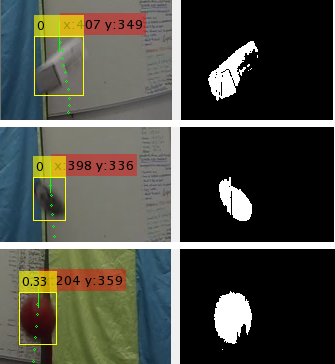
\includegraphics[width=6cm]{fault_background.png}
\end{center}

\begin{itemize}
\item  When a portion of the object is similar to its background, our algorithm can have some difficulties. As illustrated above, the objects appears to have some discontinuities. This could pose a problem for the ball recognition algorithm, since we rely on the shape of the object, which no longer appears to be spherical. However, in practice, this has not caused any misclassifications.

\item If the background is changing (e.g. when an object hits the cloth on the panel), the alterations can at first be confused with objects. This does happen in one of the videos, where these "blobs" are being tracked as objects:
\end{itemize}

\begin{center}
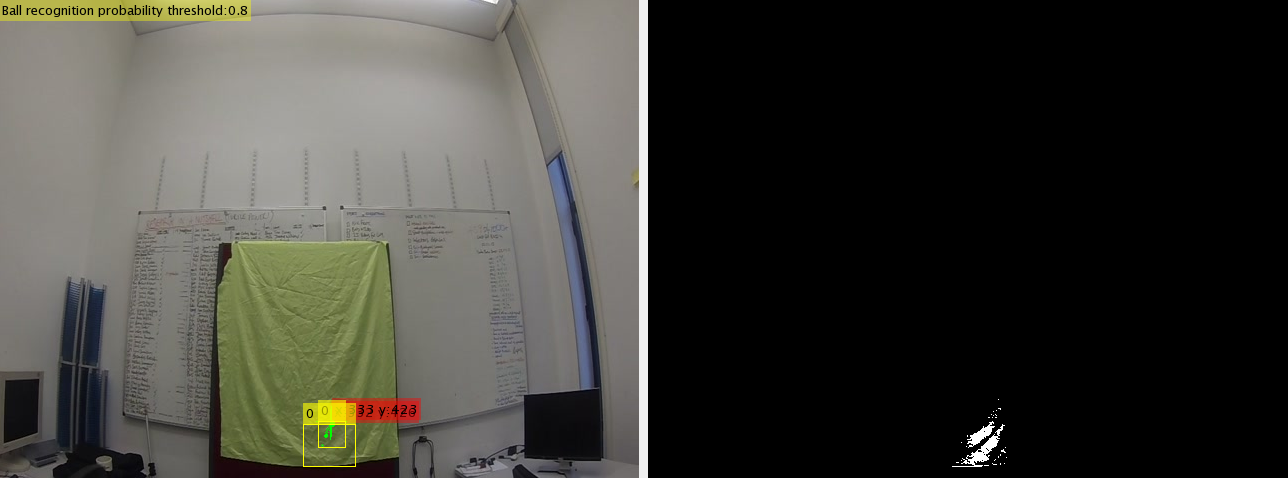
\includegraphics[width=12cm]{background_change1.png}
\end{center}
  
\paragraph{} However, we partially avoid this issue through adaptive learning, which cleans up the mask after a few iterations.

\begin{itemize}
\item Background noise is another problem that can sometimes occur. But again, it is fairly rare and does not get picked up as on object and it doesn't confuse the detection of actual objects.
\end{itemize}

\paragraph{} But generally, detection is done very reliably, as exemplified below: 
\begin{center}
	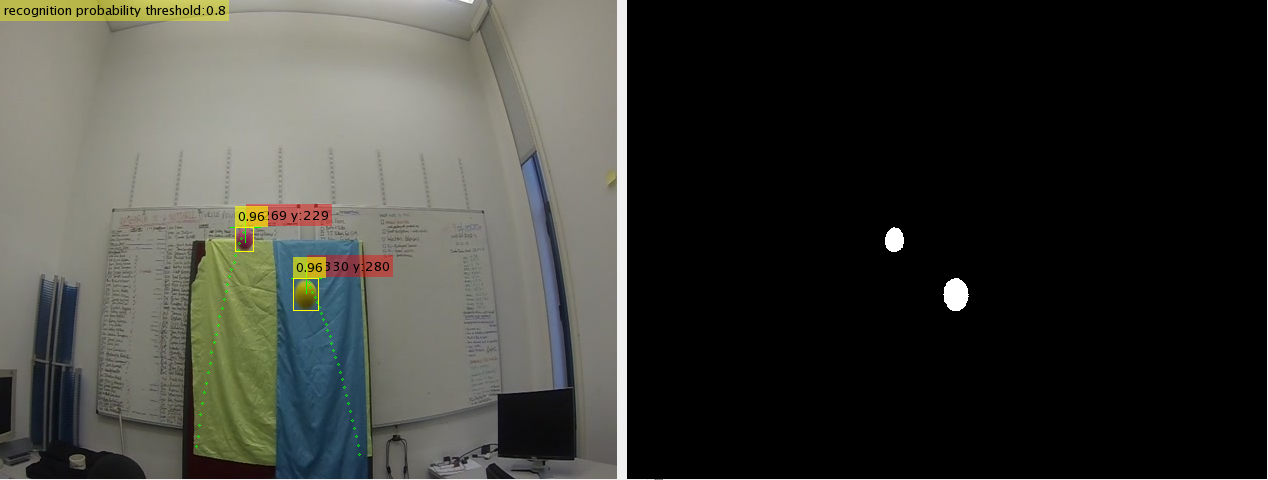
\includegraphics[width=12cm]{multi_ball_detection.png}	
\end{center}

\subsection{Object tracking and representation}

\paragraph{} The system does a good job at keeping track of which blobs correspond to which object, even when the object becomes distorted or can no longer be seen (which seems to happen fairly rarely). On the four test videos, it is perfectly accurate, being able to represent every item, almost immediately after it becomes visible until it exits the frame.

\subsection{Determining highest point}

\paragraph{} If an object is detected properly we will always find the maximum correctly. The highest point marker may not be drawn if we misclassify an object, however, the actual highest point algorithm still performs the same.
\paragraph{} For this assignment we made the assumption that the highest point an object reaches is in fact the highest (or lowest in Matlab coordinate system) point in the bounding box. This means that the highest point draw will be the top middle point of the bounding box.

\subsection{Ball recognition}

\paragraph{}	As outlined in the Methods section, we have tried a number of different approaches to ball classification. All of these rely on some parameters or threshold to be set so the calibration of these values is an important step in ensuring accurate detection. We have done this simply by experiment, trying to get the best accuracy we could on the test videos, while trying to avoid overfitting.

\paragraph{} The algorithms generally perform well. The highest confidence of classification is actually achieved on the toy kangaroos, which often get a null probability of being a ball. Conversely, smaller balls usually get classified very accurately (confidence close to 1). Rugby balls are somewhat harder, but they still get reliably classified as non-balls. The only real issues our approach has is with larger ball and small cubes. The shortcomings in this area are mostly due to the masking. We experimented with some filters in order to smooth the corners, but they came with a high computation cost and, at least with the settings that we tried, did not provide any real results.
\paragraph{} Nonetheless, accuracy is very high. Out of 22 balls across all 4 videos, we successfully detect 20 of them.

\subsection{Processing speed}
\paragraph{} In order to measure the speed of our classifier, we divide the number of frames by the number of seconds it took to finish the video to report the frame per second rate (FPS). We also subtract the the 3 second pause for each detected ball from the total time.
\paragraph{}
\centerline{
\begin{tabular}{|c|c|c|c|c|}
\hline
Video speed & GOPR002 & GOPR004 & GOPR005 & GOPR008 \\
\hline
Frames per second & 17.1 & 17.8 & 15.9 & 16.6 \\
\hline
\end{tabular}}

\paragraph{}

\subsection{Performance statistics}

%\begin{table} [!htb]
%\vspace{2mm}
\centerline{
\begin{tabular}{|c|c|c|c|c|}
\hline
Test case & GOPR002 & GOPR004 & GOPR005 & GOPR008 \\
\hline  \hline
Ratio of detected to present & 9/9 & 8/8 & 10/10 & 11/11 \\
\hline
Successfully detected & 9 & 8 & 9 & 11 \\
\hline
Non-objects detected & 2 & 0 & 0 & 0 \\
\hline
Incorrectly tracked objects & 0 & 0 & 1 & 0 \\
\hline 
\textit{Overall success rate} & \textit{88.88\%} & \textit{100\%} & \textit{100\%}  & \textit{88.88\%} \\
\hline
\end{tabular}}
%\end{table}

\paragraph{}
\paragraph{}

%\vspace{2mm}
\centerline{
\begin{tabular}{|c|c|c|c|c|}
\hline
Object classification & GOPR002 & GOPR004 & GOPR005 & GOPR008 \\
\hline  \hline
Balls correctly classified & 83.33\% & 100\% & 100\% & 87.5\% \\
\hline
Non-balls correctly classified & 100\% & 100\% & 75\% & 100\% \\
\hline 
\textit{Overall success rate} & \textit{88.88\%} & \textit{100\%} & \textit{90\%}  & \textit{81.81\%} \\
\hline
\end{tabular}}

\paragraph{}

%\vspace{2mm}
\centerline{
\begin{tabular}{|c|c|c|c|c|}
\hline
Object misclassification & GOPR002 & GOPR004 & GOPR005 & GOPR008 \\
\hline  \hline
Cubes & 0/1 & 0/2 & 1/1 & 0/1 \\
\hline 
Boxes & 0/0 & 0/0 & 0/1 & 0/1 \\
\hline 
Toys & 0/1 & 0/1 & 0/2 & 0/0 \\
\hline 
Rugby balls & 0/1 & 0/1 & 0/0 &01/1 \\
\hline 
\end{tabular}}

\paragraph{}

%\vspace{2mm}
\centerline{
\begin{tabular}{|c|c|c|c|c|}
\hline
Confidence intervals & GOPR002 & GOPR004 & GOPR005 & GOPR008 \\
\hline  \hline
Correctly classified with probability 0.9-1 & 4/6 & 4/4 & 5/6 & 6/8 \\
\hline 
Correctly classified with probability 0.8-0.89 & 1/6 & 0/4 & 1/6 & 0/8 \\
\hline 
\end{tabular}}

\begin{multicols}{2}
\section{Discussion}

\paragraph{} One area the algorithm could be improved in is automatic threshold estimation. Algorithms such as maximum likelihood could be used to attempt this. This would require a larger dataset and a way to evaluate detections either by human or to construct the videos such that the correct detections are know.
\paragraph{} Adaptive learning rate for the Foreground Detector could be improved as well in order to allow the model to adjust to changes in light and background movements such as in the first video feed provided.
\paragraph{} Furthermore, use of other features provided by the moments of an image could be used to make detection more robust. For example, color could be used to ensure the same blobs are linked together correctly consecutive frame.
\paragraph{} The algorithm we  implemented is fairly robust and works quite well overall. It manages to distinguish the balls from the rotating cubes which appears to be the most difficult task of all as the cube in motion is quite similar to a ball. Detection of toys is very accurate and in the test data is always classified as "not a ball". Detection of rugby balls is very accurate as well, the minor and major axes make it an easy task classify it as "not a ball".

\section{Work distribution}

We have collaborated on the assignment evenly and thus the split should be 50:50.

\begin{itemize}
\item \textit{Milan - } I have worked on the highest point detection and correctly pausing the video. Additionally, I have researched how the Foreground Detector works to understand how to configure it properly. On top of that, I have researched and used Matlab toolbox functions such as Blob Analysis. Further, I worked on getting the path of the ball drawn in the GUI and optimizations for the removal of tracks to ensure we do not mis-detect.
\item \textit{Victor - } Before deciding to build our system using the tutorial from \cite{ES2} I did some experimentation with background subtraction and normalization. After that, I worked on setting up our project using ideas and code from the tutorial, in order to make it work with our video streams. I then worked on our algorithm for classifying objects as balls, trying out different techniques and criteria.
\item \textit{Together - } We looked into how to best link detected blobs in a mask together with the previous images and ended up using the \texttt{assignDetectionsToTracks()} function to solve the assignment problem. Furthermore, we collaborated on design decisions and displaying the relevant information on top of the video stream.
\end{itemize}

\end{multicols}

\bibliographystyle{IEEEtran}
\begin{thebibliography}{10}
\bibitem[1]{ES1} \textit{T. Bouwmans, F. El Baf, B. Vachon} (November 12, 2008) Background Modeling using Mixture of Gaussians for Foreground Detection - A Survey \url{http://hal.archives-ouvertes.fr/docs/00/33/82/06/PDF/RPCS_2008.pdf} (Last Visited on March 5, 2014)
\bibitem[2]{ES2} \textit{Unknown Author} (Unknown Publication Date) Motion-Based Multiple Object Tracking - Matlab \url{http://www.mathworks.co.uk/help/vision/examples/motion-based-multiple-object-tracking.html} (Last Visited on March 5, 2014)
\end{thebibliography}


\section*{Full code}

\begin{verbatimtab}[2]
function multiObjectTracking(file_dir)

	% Needs to be there in order to avoid some Matlab bug.
	ones(10)*ones(10);

	% Display video
	obj.videoPlayer = vision.VideoPlayer('Position', [20, 400, 700, 520]);
	% obj.maskPlayer = vision.VideoPlayer('Position', [740, 400, 700, 520]);

	% Backgrond model and object detector
	obj.detector = vision.ForegroundDetector('NumGaussians', 2, ...
			'NumTrainingFrames', 25, 'MinimumBackgroundRatio', 0.8, ...
			'InitialVariance', 25*25, 'AdaptLearningRate', true, 'LearningRate', 0.0001);

	% Blob analysis and recognition
	obj.blobAnalyser = vision.BlobAnalysis('BoundingBoxOutputPort', true, ...
			'AreaOutputPort', true, 'CentroidOutputPort', true, ...
			'MajorAxisLengthOutputPort', true, 'MinorAxisLengthOutputPort', true, ...
			'EccentricityOutputPort', true, 'PerimeterOutputPort', true, ...
			'MinimumBlobArea', 200);

	% Global state variables
	reached_highest = java.util.ArrayList();

	 % Create an empty array of tracks.
	tracks = struct(...
		'id', {}, ...
		'bbox', {}, ...
		'kalmanFilter', {}, ...
		'age', {}, ...
		'totalVisibleCount', {}, ...
		'consecutiveInvisibleCount', {}, ...
		'stack', {}, ...        % ball / not ball classifications to get probability
		'max_x', {}, ...        % max point so far
		'max_y', {}, ...        % max point so far
		'last_x', {}, ...       % the last seen value
		'last_y', {}, ...       % the last seen value
		'should_pause', {}, ... % should we pause this object when it's highest?
		'stop_pausing', {}, ... % Have we paused yet?
		'track_xs', {}, ...     % past points for drawing the track
		'track_ys', {});        % past points for drawing the track

	% ID of the next track
	nextId = 1;

	% Threshold on the degree of confidence with which an object is classified as a ball
	ball_probability_threshold = 0.8;

	% image file names
	filenames = dir([file_dir '*.jpg']);

	% Detect moving objects, and track them across video frames.
	% Main loop of the program
	for k = 1 : size (filenames, 1)
		% Load an image
		frame = imread([file_dir filenames(k).name]);

		% Find objects on the image
		[areas, centroids, bboxes, mask, majora, minora, ...
		 eccentricities, perimeters] = detectObjects(frame);

		% Attempt to predict the location of objects
		predictNewLocationsOfTracks();

		% Match detected objects to existing objects
		[assignments, unassignedTracks, unassignedDetections] = detectionToTrackAssignment();

		% Update informations for each track - maximums and ball/not ball classification
		updateAssignedTracks();

		% Increment age of unassigned tracks to be considered for deletion later
		updateUnassignedTracks();

		% Delete the tracks that are too old or not visible
		deleteLostTracks();

		% Create new objects from unassigned tracks
		createNewTracks();

		% Draw GUI
		displayTrackingResults();
	end

	function [areas, centroids, bboxes, mask, majora, ...
			  minora, eccentricities, perimeters] = detectObjects(frame)
		% Detect foreground.
		mask = obj.detector.step(frame);

		% Perform blob analysis to find connected components.
		[areas, centroids, bboxes, majora, minora, ...
		eccentricities, perimeters] = obj.blobAnalyser.step(mask);
	end

	function predictNewLocationsOfTracks()
		for i = 1:length(tracks)
			bbox = tracks(i).bbox;

			% Predict the current location of the track.
			predictedCentroid = predict(tracks(i).kalmanFilter);

			% Shift the bounding box so that its center is at
			% the predicted location.
			predictedCentroid = int32(predictedCentroid) - bbox(3:4) / 2;
			tracks(i).bbox = [predictedCentroid, bbox(3:4)];
		end
	end

	function [assignments, unassignedTracks, ...
			  unassignedDetections] = detectionToTrackAssignment()

		nTracks = length(tracks);
		nDetections = size(centroids, 1);

		% Compute the cost of assigning each detection to each track.
		cost = zeros(nTracks, nDetections);
		for i = 1:nTracks
			cost(i, :) = distance(tracks(i).kalmanFilter, centroids);
		end

		% Solve the assignment problem.
		costOfNonAssignment = 20;
		[assignments, unassignedTracks, unassignedDetections] = ...
			assignDetectionsToTracks(cost, costOfNonAssignment);
	end

	function updateAssignedTracks()
		numAssignedTracks = size(assignments, 1);
		balls = isBall(eccentricities, perimeters, bboxes, majora, minora, areas);

		% Iterate over all the tracks we currently have assigned
		for i = 1 : numAssignedTracks
			idx = assignments(i, 1);
			detectionIdx = assignments(i, 2);
			centroid = centroids(detectionIdx, :);
			bbox = bboxes(detectionIdx, :);

			% Correct the estimate of the object's location
			% using the new detection.
			correct(tracks(idx).kalmanFilter, centroid);

			% Replace predicted bounding box with detected
			% bounding box.
			tracks(idx).bbox = bbox;

			% Update track's age.
			tracks(idx).age = tracks(idx).age + 1;

			% Update track stats
			x = bbox(1) + floor(bbox(3) / 2);
			y = bbox(2);

			% Calculate delta - the change in y coordinates
			% If checks are to exclude newly initialized objects.
			if tracks(idx).last_y ~= Inf && tracks(idx).last_y ~= -1
				deltaY = tracks(idx).last_y - y;
			else
				deltaY = 1;
			end

			% Re-assign values if current max
			if y < tracks(idx).max_y
				tracks(idx).max_x = x;
				tracks(idx).max_y = y;
			end

			% Draw only for positive values
			if tracks(idx).max_y > 0 && tracks(idx).max_y < Inf
				text = strcat('x:', int2str(tracks(idx).max_x), ' y:', int2str(tracks(idx).max_y));
				if ((~reached_highest.contains(tracks(idx).id)) || ...
					(reached_highest.contains(tracks(idx).id) && tracks(idx).should_pause))
					frame = insertMarker(frame, [tracks(idx).max_x, tracks(idx).max_y], 'Size', 15);
					frame = insertText(frame, [tracks(idx).max_x + 1, tracks(idx).max_y - 23], ...
					                  text, 'FontSize', 13, 'BoxColor', 'red', 'BoxOpacity', 0.4);
				end
			end

			% Update last frame cache
			tracks(idx).last_x = x;
			tracks(idx).last_y = y;

			% Update visibility.
			tracks(idx).totalVisibleCount = ...
				tracks(idx).totalVisibleCount + 1;
			tracks(idx).consecutiveInvisibleCount = 0;

			tracks(idx).stack.add(balls.get(i - 1));

			% Determine if we should be pausing for this object
			tracks(idx).should_pause = false;
			if deltaY < 0 && ~reached_highest.contains(idx)
				% Only pause if the probabilty of being a ball given the past is past the threshold
				if getBallProbability(tracks(idx).stack) > ball_probability_threshold
					tracks(idx).should_pause = true;
				else
					if ~reached_highest.contains(tracks(idx).id)
						reached_highest.add(tracks(idx).id);
					end
				end
			end

			% Add current location to the history of location
			tracks(idx).track_xs.add(bbox(1) + floor(bbox(3) / 2));
			tracks(idx).track_ys.add(bbox(2) + floor(bbox(4) / 2));

			% Check how many track points there are in the object
			numTracks = tracks(idx).track_ys.size();
			points = zeros(numTracks, 2);

			% Precompute a [numTracks x 2] matrix to draw markers
			for i = 1 : tracks(idx).track_ys.size()
				points(i, 1) = tracks(idx).track_xs.get(i-1);
				points(i, 2) = tracks(idx).track_ys.get(i-1);
			end

			% Draw points
			frame = insertMarker(frame, points, 'o', 'Size', 1);
		end
	end

	function updateUnassignedTracks()
		for i = 1:length(unassignedTracks)
			ind = unassignedTracks(i);
			tracks(ind).age = tracks(ind).age + 1;
			tracks(ind).consecutiveInvisibleCount = ...
				tracks(ind).consecutiveInvisibleCount + 1;
		end
	end

	function deleteLostTracks()
		if isempty(tracks)
			return;
		end

		invisibleForTooLong = 4;
		ageThreshold = 8;

		% Compute the fraction of the track's age for which it was visible.
		ages = [tracks(:).age];
		totalVisibleCounts = [tracks(:).totalVisibleCount];
		visibility = totalVisibleCounts ./ ages;

		% Find the indices of 'lost' tracks.
		lostInds = (ages < ageThreshold & visibility < 0.6) | ...
			[tracks(:).consecutiveInvisibleCount] >= invisibleForTooLong;

		% Delete lost tracks.
		tracks = tracks(~lostInds);
	end

	function createNewTracks()
		centroids = centroids(unassignedDetections, :);
		bboxes = bboxes(unassignedDetections, :);

		for i = 1:size(centroids, 1)

			centroid = centroids(i,:);
			bbox = bboxes(i, :);

			% Create a Kalman filter object.
			kalmanFilter = configureKalmanFilter('ConstantVelocity', ...
				centroid, [200, 50], [100, 25], 100);

			% Create a new track.
			newTrack = struct(...
				'id', nextId, ...
				'bbox', bbox, ...
				'kalmanFilter', kalmanFilter, ...
				'age', 1, ...
				'totalVisibleCount', 1, ...
				'consecutiveInvisibleCount', 0, ...
				'stack', java.util.ArrayList(), ...
				'max_x', -1, ...
				'max_y', Inf, ...
				'last_x', -1, ...
				'last_y', Inf, ...
				'should_pause', false, ...
				'stop_pausing', false, ...
				'track_xs', java.util.ArrayList(), ...
				'track_ys', java.util.ArrayList());

			% Add it to the array of tracks.
			tracks(end + 1) = newTrack;

			% Increment the next id.
			nextId = nextId + 1;
		end
	end

	function displayTrackingResults()
		% Convert the frame and the mask to uint8 RGB.
		frame = im2uint8(frame);
		mask = uint8(repmat(mask, [1, 1, 3])) .* 255;

		minVisibleCount = 8;
		if ~isempty(tracks)

			% Noisy detections tend to result in short-lived tracks.
			% Only display tracks that have been visible for more than
			% a minimum number of frames.
			reliableTrackInds = ...
				[tracks(:).totalVisibleCount] > minVisibleCount;
			reliableTracks = tracks(reliableTrackInds);

			% Display the objects. If an object has not been detected
			% in this frame, display its predicted bounding box.
			if ~isempty(reliableTracks)

				% Get bounding boxes.
				bboxes = cat(1, reliableTracks.bbox);

				% Get ids.
				ids = int32([reliableTracks(:).id]);

				% Create labels for objects indicating the ones for
				% which we display the predicted rather than the actual
				% location.
				labels = cellstr(int2str(ids'));
				for i = 1 : size(reliableTracks, 2)
					ballProb = getBallProbability(reliableTracks(i).stack);
					ballProb=round(ballProb*100)/100;
					if ~reached_highest.contains(reliableTracks(i).id)
						labels(i) = cellstr(num2str(ballProb));
					else
						if reliableTracks(i).should_pause
							labels(i) = cellstr('Ball');
						else
							labels(i) = cellstr('Not a ball');
						end
					end
				end

				predictedTrackInds = ...
					[reliableTracks(:).consecutiveInvisibleCount] > 0;
				isPredicted = cell(size(labels));
				isPredicted(predictedTrackInds) = {' predicted'};
				labels = strcat(labels, isPredicted);

				% Draw the objects on the frame.
				frame = insertObjectAnnotation(frame, 'rectangle', ...
					bboxes, labels);

				for i = 1 : size(reliableTracks, 2)
					if reliableTracks(i).should_pause && ...
					 ~reached_highest.contains(reliableTracks(i).id)
						pause(3);
						reached_highest.add(reliableTracks(i).id);
					end
				end
			end


		end

		% Display the mask and the frame.
		% obj.maskPlayer.step(mask);
		obj.videoPlayer.step(frame);

	end

	function prob = getBallProbability(stack)
		% Given a list of boolean values, calculate the ratio of true to total
		% The ratio is the confidence with which an object is classified as a ball
		%  at a particular moment in time.
		len = stack.size();
		count = 0;

		% Iterate over the values and count
		for i = 1 : len
			if stack.get(i-1)
				count = count + 1;
			end
		end

		% Calculate probability as a ratio
		prob = count / len;

		% Only consider objects that have at least 8 values
		if len < 8
			prob = 0;
		end
	end

	function balls = isBall(eccentricities, perimeters, bboxes, majors, minors, areas)
		% Determines whether a blob is spherical, based on properties output by BlobAnalysis
		% Uses eccentricity of second moment ellipses, estimated parameter of the fitting
		%  ellipse and compactness of the blob.
		balls = java.util.ArrayList();

		for i = 1 : size(eccentricities)
			if eccentricities(i) < 0.8
				estimatedRadius = (majors(i) + minors(i))/2;
				estimatedPerimeter = pi * estimatedRadius;

				ratio = perimeters(i)/estimatedPerimeter;
				if ratio < 1.2
					% Compactness
					compactness = perimeters(i)*perimeters(i)/(4*pi*double(areas(i)));
					balls.add(compactness < 1.8);
				else
					balls.add(false);
				end
			else
				balls.add(false);
			end
		end
	end

end
\end{verbatimtab}

\end{document}
